\section{Synthesis: Reliability, Hallucination, and Legal Citation Verification}
\label{sec:reliability}

The chronological account in Sections~\ref{sec:foundations}--\ref{sec:2026} raised the reliability
problem repeatedly without resolving it. \citet{dahl2024} documented fabricated authorities in 2024.
\citet{magesh2025} found hallucinations persisting in commercial legal research tools despite their
use of RAG in 2025. \citet{butler2026} proposed a formal taxonomy for telling different kinds of
failure apart in 2026. This section draws those threads together into a single account of what legal
AI reliability actually requires.

Access to external evidence does not automatically make a legal answer reliable. A system may
retrieve a relevant document but misread its meaning, miss an exception, cite the wrong passage, or
draw a conclusion the retrieved evidence does not support. Legal correctness depends on more than
textual similarity. An answer can accurately reproduce a sentence from a judgment while still
misrepresenting its holding. It can identify the correct statute while missing an amendment or
jurisdictional restriction that affects its application. We can organize reliability around three
related questions, and none of them can stand in for the others. Did the system retrieve the right
evidence? Does the evidence support the claim, rather than merely discuss a similar topic? Does the
claim apply legally, given the jurisdiction, date, and procedural context?

\citet{butler2026} gave this last distinction a precise, testable form. Instead of reporting one
aggregate accuracy score, their hierarchical error-decomposition taxonomy, reproduced in
Figure~\ref{fig:rag-errors}, separates three failure modes. It uses three binary signals the authors
collected per question, embedding model, and LLM.

% Figure reproduced from Butler and Butler (2026), "Legal RAG Bench: An End-to-End
% Benchmark for Legal RAG", Figure 1, for scholarly discussion and critique within this
% review. Copyright remains with the original authors/publisher.
\begin{figure*}[t]
\centering
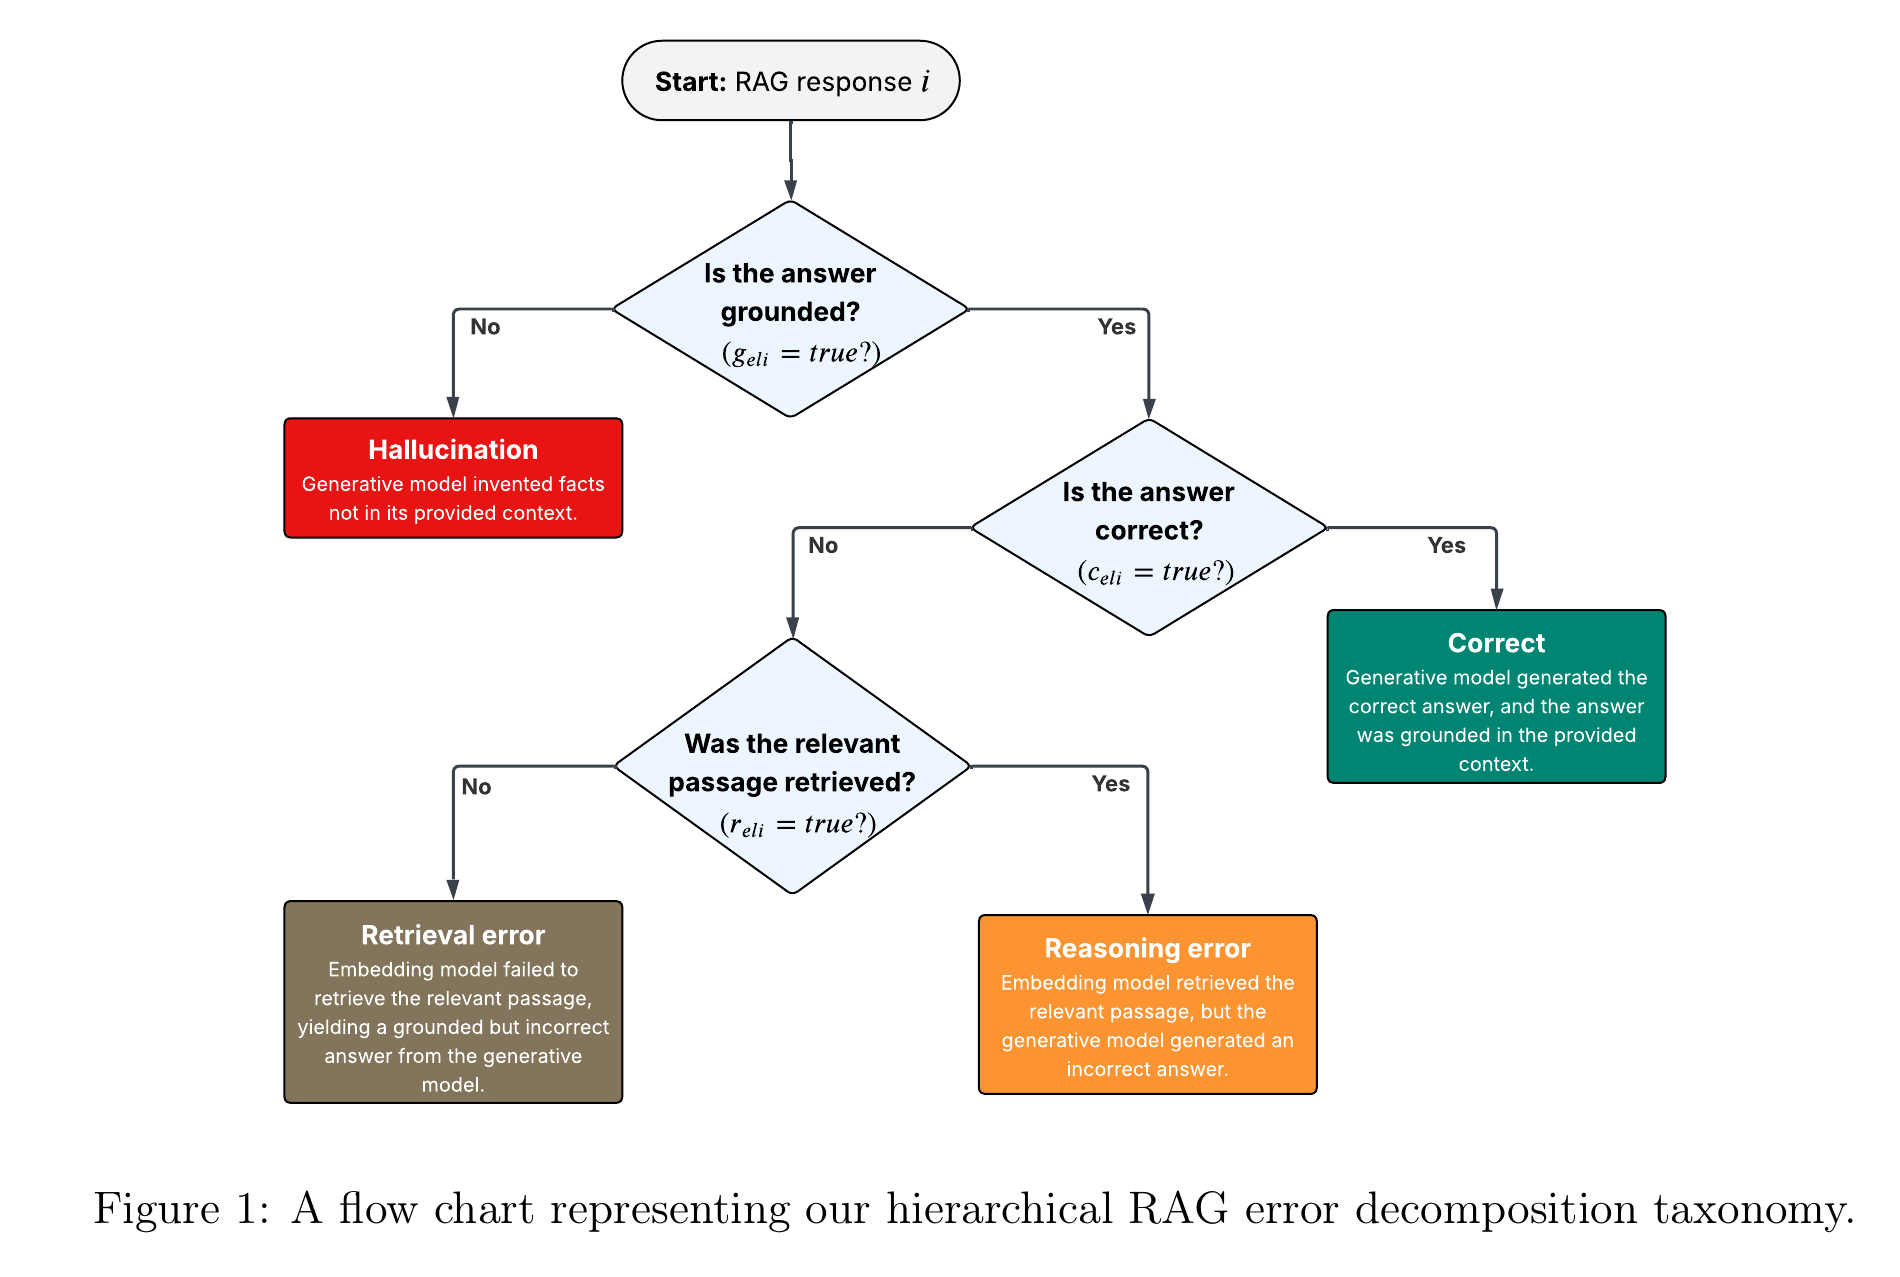
\includegraphics[width=\textwidth]{images/butler2026_fig1.png}
\caption{Figure reproduced from \citet{butler2026}: the hierarchical RAG error-decomposition
taxonomy. Rather than reporting one aggregate accuracy score, the taxonomy separates three
distinct failure modes using three binary signals collected per question, embedding model, and
LLM: groundedness ($g$, whether the answer is supported by what was retrieved), retrieval
accuracy ($r$, whether the annotated supporting passage was actually retrieved), and correctness
($c$, whether the answer entails the reference answer). This distinguishes an ungrounded
hallucination from a grounded answer that is wrong because retrieval failed, and from a grounded,
correctly retrieved answer that the generator still reasoned about incorrectly.}
\label{fig:rag-errors}
\end{figure*}


An ungrounded \textbf{hallucination}, where what the system retrieved does not support the answer,
differs from a grounded answer that is wrong because the system never retrieved the needed passage,
a \textbf{retrieval error}. Both differ again from a grounded, correctly retrieved answer that the
generator still reasoned about incorrectly, a \textbf{reasoning error}. This distinction matters in
practice, because it determines what fixing the system actually requires. A hallucination calls for
stronger grounding and abstention. A retrieval error calls for a better retriever or a richer index.
A reasoning error calls for improving how the generator uses the evidence it already has.
Table~\ref{tab:failures} extends this taxonomy with the broader set of reliability failures this
survey has encountered across its chronology.

\begin{table*}[tp]
\centering
\caption{Reliability failure modes in legal AI and possible mitigations.}
\label{tab:failures}
\footnotesize
\setlength{\tabcolsep}{5pt}
\renewcommand{\arraystretch}{1.25}
\begin{tabularx}{\textwidth}{>{\raggedright\arraybackslash}p{2.6cm} >{\raggedright\arraybackslash}X >{\raggedright\arraybackslash}X}
\toprule
\textbf{Failure type} & \textbf{Description} & \textbf{Possible mitigation} \\
\midrule
Hallucination \citep{dahl2024, butler2026} & The system invents a case, statute, or citation, or asserts a claim the retrieved evidence does not support. & Citation resolution against authoritative databases; abstention when evidence is missing. \\
Retrieval error \citep{butler2026} & The answer is grounded in retrieved text, but the system never retrieved the passage it actually needed. & A better retriever, hybrid retrieval, or a richer structure-aware index. \\
Reasoning error \citep{butler2026} & The system retrieved the correct passage, but the generator still drew an incorrect conclusion from it. & Claim-to-passage entailment checking and role-aware judgment analysis. \\
Incomplete evidence & The system retrieved a relevant exception, counter-authority, or condition only partially. & Query expansion and retrieval of related provisions. \\
Outdated or jurisdictionally mismatched law & The system applies a superseded or foreign authority, as the Pakistani case study in Section~\ref{sec:jurisdiction} illustrates. & Effective-date metadata and jurisdiction filtering. \\
\bottomrule
\end{tabularx}
\end{table*}

We should not treat a citation as reliable merely because it resolves to an existing document.
Verification splits into four checks. Citation resolution asks whether the cited authority exists
and whether a reader can locate it. Passage verification asks whether the cited passage actually
contains the relevant language. Claim-support verification asks whether the passage actually
supports the claim. Applicability verification asks whether the authority applies to the
jurisdiction, date, and procedural context of the question. This means verification should work at
the level of individual claims, not a whole response, since a long answer can contain several
supported statements and one unsupported conclusion that a document-level check would miss.
\citet{pipitone2024}'s focus on retrieving precise text segments, introduced in
Section~\ref{sec:rag2024}, reinforces the importance of granular evidence. Precise retrieval and
legal entailment still remain separate requirements, though: finding the correct passage does not by
itself show that the generated interpretation of it is valid. We should not read either
\citet{dahl2024} or \citet{magesh2025} as establishing one universal hallucination rate. Results
depend on the tools, tasks, jurisdictions, and definitions of error each evaluation uses. That is
why a reproducible evaluation should disclose the corpus's jurisdiction and temporal scope, the
source of its test questions, the operational definition of hallucination it uses, and the
annotation protocol and reviewer expertise behind its results, in the spirit of the groundedness,
retrieval-accuracy, and correctness signals \citet{butler2026} report separately instead of folding
into one number.

Multiple safeguards handle reliability better than any single verification component. These
include authoritative source management that records provenance, jurisdiction, and effective dates.
They include retrieval and ranking across the lexical, dense, and structure-aware methods described
in Section~\ref{sec:rag2024}. They include claim-level generation that ties each material assertion
to a supporting passage. They include verification that resolves citations and tests claim support.
And they include a qualified response or abstention when evidence is missing or contradictory. We
put this conceptual workflow together for this survey; it is not a claim that every reviewed system
implements all five stages. Agentic architectures, such as the one Legalyze uses in
Section~\ref{sec:2026}, can coordinate these safeguards, but adding agents does not automatically
improve correctness. If the agents share the same incomplete corpus, or repeat the same unsupported
assumption, orchestration can reproduce the underlying error instead of correcting it. The central
lesson of this chapter, and arguably of this entire survey, is that legal AI reliability demands an
evidence-to-claim evaluation. A dependable system must retrieve appropriate authority, keep its
context, generate claims that follow from the evidence, verify citations, and recognize when legal
applicability remains uncertain.
